\chapter{\label{ch:theoretical_framework} Theoretical Framework}

Classical computers are Turing devices and therefore, depend on discrete set of instructions that cannot represent the intrinsic duality and probabilistic nature of quantum particles. For example, sampling quantum information in discrete time intervals could introduce errors to the system. The properties of quantum particles, which form the foundation of quantum information processing systems, are detailed in the following section. Transistors used to implement classical systems take advantage of the quantum mechanical phenomena that occur when electrons and holes transition between the energy levels of semiconductor substrates, however, this application of quantum mechanics does not directly exploit the properties of superposition, entanglement and interference of the quantum states that are required to realise quantum computer. Since the elementary unit of information in quantum computers is a qubit which represent the quantum state of particles in the system, the chapter begins by introducing the notion of quantum states through the \textit{Born postulate} that associates a probabilistic wave function to a quantum particle such as a photon, electron or exciton. 

A concrete mathematical formulation of quantum states is necessary for implementing the QFT which forms an essential part of the phase estimation procedure that is crucial in the design of the emulated quantum computer. This chapter also introduces the concept of Hilbert spaces and the transformations associated with single-qubit and two-qubit quantum gates to describe the QFT as a quantum circuit that represents a sequence of unitary operations performed on a quantum state. The QFT is of particular interest for its application as a subroutine in the Shor's factoring algorithm on the FPGA. The subroutine of interest in the emulation of the quantum search algorithm is the quantum oracle, which behaves like a black box with unexposed operations that prepare an unknown state. For each algorithm, an example of the 3-qubit quantum circuit is shown to illustrate the quantum gate operations that are necessary.

Overall, the theoretical framework begins with the postulates of quantum mechanics, followed by introduction to quantum states and Hilbert spaces, unitary operations. Following the mathematical description, the concept of qubits as quantum states that represent quantum information is introduced. The section culminates in a detailed description of phase estimation and its applications in the QFT and Shor's quantum factoring algorithm. Further elaboration on the quantum search algorithm is also included. Finally, a conclusion is drawn to summarise the theoretical background and its relevance to emulating a quantum computing on a FPGA. 

\section{Quantum Mechanics \label{sec:q_mechanics}}

\subsection{Postulates of Quantum Mechanics \label{subsec:uncertain_quant_dual}}

Quantum computing is based on the underlying principles of information theory and quantum mechanics. While this is also true for classical computers in that quantum mechanics principles govern the flow of electrons in the transistors contained in classical semiconductor chips, the influence of quantum mechanics in quantum computing extends beyond low-level implementation to the domain of computation and communication \cite{Rieffel2011}. This applicability of the subject of quantum mechanics in both quantum computing and classical computing is because the subject seeks to describe the behaviour of atomic and subatomic particles, or quantum particles, such as electrons, protons and photons. 

Classical mechanics fails to fully describe the behaviour of quantum particles. Consider a system of localised particles with a mass $m_i$, where $i$ is the index of the $i$-th particle. At any given time $t$, the state of the system of particles can be described by a set of position vectors, $\mathbf{r}_i$, and linear momenta $\mathbf{p_i}$. Given that the mass, position and momentum of each particle can be measured with high precision, the principles of classical mechanics suggest that progression of the state of the system can be determined with \textit{certainty} since the set of trajectories can be retrieved from an application of Newton's equation of motion which is defined by an initial value system of differential equations 
\begin{align}
	\mathbf{F}_i	& = m_i \frac{d^2 \mathbf{r}_i}{dt^2} = \frac{d}{dt} \mathbf{p}_i
\end{align}
where $F_i$ is the force experience by particle $i$ at time $t$. 

The implication that the universe is deterministic that stems from an interpretation of Netwon's equations of motion pointed to many deficiencies in classical mechanics. The first deficiency in classical mechanics that is addressed in quantum mechanics involves the \textit{uncertainty} in measurements. Using a thought experiment, Max Born highlighted that there is an inherent uncertainty in determining the position of an electron through a microscope due to optics. There is also an inherent uncertainty about the momentum of the electron since the photon which is released by the electron and observed through the microscope lens because of there is an uncertainty in the directional component. The relationship between the uncertainty in the position and the momentum of the particle expounded by the \textit{Heisenberg's Uncertainty Principle} which states that given an uncertainty in position, $\Delta x$, and an uncertainty in the momentum, $\Delta p$, the inequality
\begin{align}
	\Delta x \Delta p & \geq \hbar
\end{align}
where $\hbar = h/2\pi$ (and $h$ is Planck's constant). Intuitively, this inequality implies that the position and momentum of a quantum particle cannot be known exactly. Gaining information about the position of a quantum particle introduces uncertainties in the momentum. Conversely, gaining information about the momentum of a particle in a quantum system leads to uncertainties in the position of that particle.

Another discrepancy in the application of classical mechanics to quantum particles arises when considering the atomic model. From the perspective of classical mechanics, an electron in a hydrogen atom would lose kinetic energy as its orbitals collapses into a spiral that terminates at the nucleus of the atom. In other words, classical mechanics suggests that the energy of the electron is continuous. However, quantum mechanics suggests that quantum particles have discrete amounts of energy in each atomic orbital. 

Quantum mechanics also addresses classical mechanic's inability to elucidate the duality of quantum particles. Young's double slit experiment and known phenomena, such as the photoelectric effect and Compton scattering, expose the wave-particle nature of photons and electrons that allows them behave like waves or particles, depending on the experiment. 

\subsection{Quantum States \label{subsec:q-states}}


To reconcile with the Heisenberg's Uncertainty Principle, energy quantisation, and wave-particle duality, quantum mechanics associates a particle with a probability wave denoted by $\psi$. Born postulated that the probability, $P(x,y,z,t)dxdydz$, of finding a particle in the infinitesimal volume, $dxdydz$, at time $t$, is proportional to the magnitude of the state function $\psi$. This state function $\psi$, or \textit{quantum state}, contains all of the information that describes the quantum system. A quantum state must satisfy the normalisation property which states that
\begin{align}
	\int_{\tau} \psi^* (\mathbf{r}, t) \psi(\mathbf{r}, t) & = 1 
\end{align}
where $\tau$ is the domain in which measurements of the state are taken.

In this paper, a quantum system is regarded as a system consisting of a one or more quantum particles that is fully defined by the quantum state function $\psi$. To define the quantum state of a particle more succinctly, consider the case where a single photon that is projected through a polarising gradient. The circular polarisation of the photon is considered to be the state of the quantum system. The state of a quantum system can be in a \textit{superposition} of the vertical polarisation, $\ket{\uparrow}$, and the horizontal polarisation, $\ket{\rightarrow}$. By expressing each polarisation state as a unit vector, the measurement of a quantum state $\psi$ can be written as a linear combination of the horizontal and vertical bases, $\ket{\uparrow}$ and $\ket{\rightarrow}$, respectively, as
\begin{align}
	\ket{\psi}	& = \alpha \ket{\uparrow} + \beta \ket{\rightarrow}
\end{align} 
where the coefficients $\alpha$ and $\beta$ are complex amplitudes of the state that satisfy the property 
\begin{align}\label{eqn:normalisation-condition}
	|\alpha|^2 + |\beta|^2	& = 1
\end{align}
The measured quantum state $\psi$ can be mapped to a unit circle where the angle subtended by the horizontal polarisation direction and the state unit vector corresponds to the measured polarisation angle. The quantum state of the photon can be illustrated as shown in figure \ref{fig:photon-polarization-circle} and is said to be in \textit{superposition} if the amplitude coefficients are both non-zero, i.e. the photon is polarised horizontally and vertically simultaneously. 
\begin{figure}
	\centering
	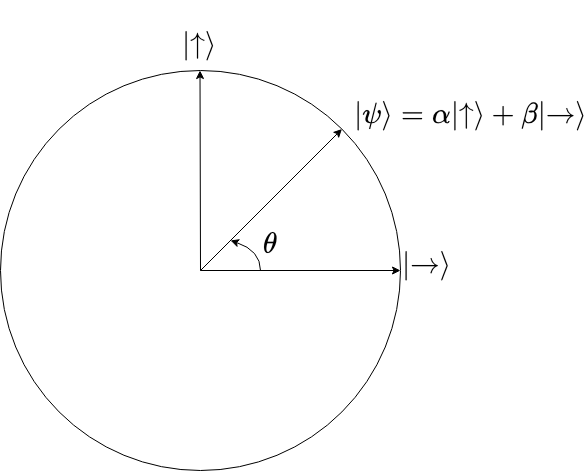
\includegraphics[width=0.45\linewidth]{body/ch2/figs/photon-polarization-circle}
	\caption[Graphical Representation of a Photon Polarisation State.]{A photon can be polarised vertically with probability $|\alpha|^2$ or horizontally with probability $|\beta|^2$. As a consequence of the probability normalisation condition, pure quantum states can be represented graphically on a unit circle as illustrated.}
	\label{fig:photon-polarization-circle}
\end{figure}
If the preferred axis of the polarising gradient is $\ket{\rightarrow}$, the photon is absorbed with a probability of $|\alpha|^2$ and passes through with a probability of $|\beta|^2$. Therefore, the probability that the photon passes through the polariser is the square of the magnitude of the amplitude coefficients in the direction of the preferred axis \cite{Rieffel2011}.

\subsection{Unitary Operations on Quantum States \label{subsec:unitary-ops}}

The analysis of the polarisation state of the quantum system with a single photon explored above can be extended to quantum systems that can be in $N$ different, mutually exclusive classical states. In this case, a quantum state is a superposition of classical states in the form

\begin{align}
	\ket{\psi}	& = \alpha_0 \ket{0} + \alpha_1\ket{1} + ... + \alpha_{N-1} \ket{N-1}
\end{align}
Superposition implies that state $\ket{\psi}$ is in each state $\ket{i}$ with amplitude $\alpha_i$. The vector space $\{\ket{0}, \ket{1}, ..., \ket{N-1}\}$ of states consists of unit vectors that are orthogonal to each other and therefore forms an $N$-dimensional orthonormal basis of a \textit{Hilbert space}, i.e. the vector space of quantum states has an inner product \cite{DeWolf2019}. Thus, a quantum state $\psi$ is a vector in Hilbert space, herein expressed as an $N$-dimensional column vector
\begin{align}
	\ket{\psi}	& = \left(\begin{matrix}
		\alpha_{1} \\
		\alpha_{2} \\
		\vdots \\
		\alpha_{N-1}
	\end{matrix}\right)
\end{align}
with the conjugate transpose
\begin{align}
	\bra{\psi}	& = (\alpha_{0}^{*}, \alpha_{1}^{*}, \hdots, \alpha_{N-1}^{*})
\end{align}
Suppose that the state unit vectors $\ket{0}, \ket{1}, \hdots, \ket{N-1}$ form the orthonormal basis of the Hilbert space $\mathcal{H}_A$, and $\ket{0}, \ket{1}, \hdots, \ket{M-1}$ form an orthonormal basis $\mathcal{H}_B$. The Hilbert spaces $\mathcal{H}_A$ and $\mathcal{H}_B$ can be combined using in a tensor product Hilbert space $\mathcal{H}$, defined as
\begin{align}
	\mathcal{H}	& = \mathcal{H}_A \otimes \mathcal{H}_B 
\end{align}
The output tensor product space has $N\cdot M$ dimensions spanned by the set of states $S_{\mathcal{H}}$, given by
\begin{align}
 S_{\mathcal{H}}	& = \{\ket{a} \otimes \ket{b}\}
\end{align}
where $a \in \{0,1,\hdots, N-1\}$ and $ b \in \{0,1,\hdots, M-1\}$. Thus, any quantum state $\ket{\psi}_{\mathcal{H}}$ in the combined Hilbert space $\mathcal{H}$ can be expressed as the sum
\begin{align}
	\ket{\psi_\mathcal{H}} & = \sum_{i=0}^{N-1}\sum_{j=0}^{M-1} \alpha_{ij} \ket{a_i} \otimes \ket{b_j}
\end{align}
called a \textit{bipartite} quantum state \cite{DeWolf2019}. Although there are higher dimensional tensor products Hilbert space of multiple states, this paper focuses on the operation and simulation of bipartite states.

A linear operation can be performed on a state $\ket{\psi}$ to change it to a different state, $\phi$, Applying the $N \times N$ complex-valued \textit{unitary operation} $U$ on the vector space of the state $\ket{\psi}$ maps it to the space of state $\ket{\phi}$. Formally, a unitary operator is a bounded linear mapping 
\begin{align}
	U: \mathcal{H} \rightarrow \mathcal{H}
\end{align}
on the Hilbert Space $H$ that preserves the norm, and satisfies
\begin{align}
	U^{*}U	& = UU^{*} = I
\end{align}
where $U^{*}$ is the Hermitian adjoint of $U$, and $I$ is the identity operator. The corollary is that a matrix $U$ is \textit{unitary} if 
\begin{align}
	U^{-1}	& = U^{*}
\end{align}
,i.e. if the inverse of $U$ is equal to the complex adjoint of $U$. The linear operator $U$ on the Hilbert space $\mathcal{H}$ defines a Hermitian adjoint operator $U^{*}$ on the space that obeys the rule
\begin{align}
	\braket{Ux, y} & = \braket{x, U^{*}y}
\end{align}
where $\braket{\cdot, \cdot}$ is the inner product on $\mathcal{H}$. Another property of the unitary matrix that can be derived from its definition is that the determinant of $U$ is can be mapped to a unit circle in the complex plane, i.e.
\begin{align}
	|det(U)|	& = 1 
\end{align}
Given an outcome state
\begin{align}
	\phi	& = \beta_0\ket{0} + \beta_1\ket{1} + \hdots + \beta_{N-1}\ket{N-1}
\end{align}
with a probability constraint
\begin{align}
	\sum_{j=0}^{N-1} |\beta_j|^2	& = 1
\end{align}
the unitary transformation $U$ that is applied to $\psi$ can be expressed as the matrix multiplication
\begin{align}
	\ket{\phi}	& = U\ket{\psi}\nonumber\\
	\ket{\phi} & = \left(\begin{matrix}
		u_{11} & u_{12} & \hdots & u_{1N}\\
		u_{21} & u_{22} & \hdots & u_{2N}\\
		\vdots & \vdots & \vdots & \vdots\\
		u_{N1} & u_{N2} & \hdots & u_{NN}
	\end{matrix}\right) 	\left(\begin{matrix}
	\alpha_{1} \\
	\alpha_{2} \\
	\vdots \\
	\alpha_{N-1}
\end{matrix}\right)	\nonumber\\ & = \left(\begin{matrix}
\beta_{1} \\
\beta_{2} \\
\vdots \\
\beta_{N-1}
\end{matrix}\right)
\end{align}
Since the unitary operator is linear and always has an inverse, it follows that operations performed on a quantum state are reversible. That is, the initial state $\ket{\psi}$ can be retrieved by applying the inverse operator $U^{-1}$ to the state $\ket{\phi}$.  

\section{Qubits as Quantum States \label{sec:q-states-qubits}}

\subsection{Qubit Superposition in the Computational Basis}

Quantum computing extends the principles of quantum mechanics to the domain of computation. Unlike a classical bit that can be 0 or 1, but not both at the same time, a \textit{quantum bit} or \textit{qubit}, is a unit of information that can be in a superposition of 0 and 1, corresponding to a quantum state $\ket{\psi}$ of a Hilbert space with two basis states, $\ket{0}$ and $\ket{1}$. 

The basis states are associated with two orthogonal vectors
\begin{align}
	\ket{0} = \left(\begin{matrix}
		1\\
		0
	\end{matrix}\right) &, \ket{1} = \left(\begin{matrix}
	0\\
	1
\end{matrix}\right)
\end{align}
such that, at a given time $t$, a qubit in quantum state $\ket{\psi}$ can be expressed as the superposition
\begin{align}\label{eqn:qstate}
	\ket{\psi}	& = \alpha_0\left(\begin{matrix}
		1\\
		0
	\end{matrix}\right) + \alpha_1\left(\begin{matrix}
	0\\
	1
\end{matrix}\right)
\end{align}
that satisfies the normalisation constraint
\begin{align}
	|\alpha_0|^2 + |\alpha_1| & = 1
\end{align}
This implies that when a qubit in superposition is measured, it collapses with to the state $\ket{0}$ or $\ket{1}$, with a probability of $|\alpha_0|^2$ and $|\alpha_1|^2$, respectively.

\subsection{Qubit Entanglement in the Computational Basis\label{subsec:qubit-entanglement}}
Quantum systems of multiple qubits exist in two-dimensional complex Hilbert space as described in section \ref{subsec:q-states} for quantum states of $N$ particles. The $N$-dimensional tensor product space of the system contains a set of basis states with a cardinality of $2^{N}$, i.e. a system with $n$ qubits has $2^n$ basis states, each of the form
\begin{align}
	\ket{q_1}\otimes\ket{q_2}\otimes\hdots\otimes\ket{q_n}
\end{align} 
with $q_i\in \{0,1\}$. In this paper, basis states are abbreviated as $\ket{q_1 q_2 q_3 \hdots q_n}$ or written in decimal form as $\ket{1}, ~\ket{2}, \hdots, \ket{2^n -1}$, depending on the computation. A quantum system with multiple qubits is referred to as a \textit{quantum register} of $n$ qubits and is considered to be in any superposition of the $n$ states represented in decimal form as
\begin{align}\label{eqn:multiple-qubit-state}
	\ket{\psi_{qr}} & = \alpha_{0}\ket{0} + \alpha_{1}\ket{1} + \alpha_2 \ket{2} + \cdots + \alpha_{2^n - 1}\ket{2^{n-1}}
\end{align}  
for
\begin{align}
	 \sum_{i=0}^{2^n - 1} |\alpha_i|^2 & = 1 	
\end{align}
Composite systems consist of two or more quantum subsystems. Statistical ensembles of pure quantum subsystem spaces show non-classical correlations between basis states, known as \textit{quantum entanglement}.  Qubits in composite quantum systems can leverage quantum \textit{entanglement} to facilitate linear operations and classical communications (LOCC). Formally, a pure quantum state $\ket{\psi}$ is said to be entangled if it is not \textit{separable}. A separable pure state $\ket{\xi}$, in a tensor product Hilbert space $\mathcal{H}_{nm} = \mathcal{H}_n \otimes \mathcal{H}_m$, can be written as the tensor product of states $\psi~\in~\mathcal{H}_n$ and $\phi~\in~\mathcal{H}_m$, i.e.
\begin{align}
	\ket{\xi}	& = \ket{\psi}\otimes\ket{\phi}
\end{align}
Consider the pure bipartite state
\begin{align}
	\ket{\psi^+}	& = \frac{1}{\sqrt{2}}\ket{00}+\frac{1}{\sqrt{2}}\ket{11}
\end{align}
from the tensor product space $\mathcal{H}_{22} = \mathcal{H}_{2}\otimes\mathcal{H}_2$. It can be shown that this bipartite state $\ket{\psi}^+$, known as an EPR pair, is indeed entangled. Let
\begin{align}
	\ket{\psi_1}	& = \alpha\ket{0} + \beta\ket{1}\nonumber\\
	\ket{\psi_2} 	& = \gamma\ket{0} + \delta\ket{1}\nonumber
\end{align} 
be pure states from the two-dimensional Hilbert space where
\begin{align}
	|\alpha|^2 + |\beta|^2 & = 1\nonumber\\
	|\gamma|^2 + |\delta|^2 & = 1\nonumber
\end{align}
If the state $\ket{\psi}^+$ is separable, it can be written as
\begin{align}
	\ket{\psi}^+	& = \ket{\psi_1}	\otimes		\ket{\psi_2}\nonumber\\
					& = (\alpha\ket{0} + \beta\ket{1})\otimes(\gamma\ket{0} + \delta\ket{1})\nonumber
\end{align}
From the property of distributivity of the tensor product and the assumption of separability, the bipartite state $\psi^{+}$ the product above can be expanded to
\begin{align}
	\ket{\psi}^+	& = \frac{1}{\sqrt{2}}\ket{00}+\frac{1}{\sqrt{2}}\ket{11}\nonumber\\
					& = \alpha\gamma\ket{00} + \alpha\delta\ket{01} + \beta\gamma\ket{10} + \beta\delta\ket{11}\nonumber 
\end{align}
For the assumption of separability to hold true, the state amplitudes must satisfy
\begin{align}
	\alpha\delta&=\beta\gamma=0\nonumber\\
	\alpha\gamma&=\beta\delta=\frac{1}{\sqrt{2}}\nonumber
\end{align}
Since there are no values such that these statements are true, it must be that 
\begin{align}
	\ket{\psi}^+	& \neq \ket{\psi_1}\otimes\ket{\psi_2}\nonumber
\end{align}
Hence, the pure state $\ket{\psi^+}$ is entangled \cite{Kurzyk2012}. Similarly, it can be shown that the state $\ket{\psi^-}$ defined by
\begin{align}
	\ket{\psi^-}	& =  \frac{1}{\sqrt{2}}\ket{00}-\frac{1}{\sqrt{2}}\ket{00}\nonumber
\end{align}
is an entangled state.   Initially, both $\ket{\psi_1}$ and $\ket{\psi_2}$ are in a superposition of the $\ket{0}$ and $\ket{1}$ basis states. The state of the qubit collapses to $\ket{00}$ when state $\ket{\psi_1}$ is measured and $\ket{0}$ is observed. Therefore, an observation of the eigenstate $\ket{\psi_1}$ is correlated to the eigenstate $\ket{\psi_2}$ of the second qubit that was not observed.
The states $\ket{\psi^+}$ and $\ket{\psi^-}$ belong to a set of four orthogonal eigenvectors of entangled states, namely
\begin{align}
	\ket{\psi^\pm} & = \frac{1}{\sqrt{2}}\ket{00} \pm \frac{1}{\sqrt{2}}\ket{11}\\
	\ket{\phi^\pm} & = \frac{1}{\sqrt{2}}\ket{01} \pm \frac{1}{\sqrt{2}}\ket{10}
\end{align}
Entanglement in bipartite state quantum systems can be exploited using non-local quantum unitary operations. These operations are independent of the distance between entangled qubits, since information about one state in an entangled 2-qubit system simultaneously reveals information about an associated, non-classically correlated state.

The degree of qubit entanglement is quantified by the \textit{Schmidt number} whose logarithm corresponds to the zero-error entanglement cost of generating a given quantum state using LOCC \cite{Gupta2020}. Quantum information theory also uses \textit{von Neumann entropy} to quantify the extent of entangle of qubits. This is because for an system of entangled states, von Neumann entropy of a joint Hilbert space $\mathcal{H}_{nm}$ can be smaller than the entropy of its subsystems. To define von Neumann entropy, a density operator $\rho$ is assigned to a quantum system with pure state and is given by
\begin{align}
	\rho	& = \ket{\psi}\bra{\psi}
\end{align}
A mixed state is a statistical ensemble of density operators of pure states, where each density operator $\rho$ is a Hermitian projection operator which satisfies $\rho^2 = \rho$. The von Neumann entropy $\mathcal{E}$ is then defined as
\begin{align}
	\mathcal{E}(\rho)	& = -\text{tr}(\rho \log \rho)
\end{align}
The von Neumann entropy of a pure quantum state is equal to 0, and the entropy of a maximally mixed state is equal to
\begin{align}
	\mathcal{E}(\rho)	& = - \sum_{i=0}^{n} \frac{1}{n} \log \frac{1}{n} = \log n
\end{align}
Similarly, it can be shown that if $\rho_n$, $\rho_m$ and $\rho_{nm}$ are the density operators of quantum systems $\mathcal{H}_n$, $\mathcal{H}_m$, and composite system $\mathcal{H}_nm$, then the joint von Neumann entropy of the system must satisfy
\begin{align}
	\mathcal{E}(\rho_n, \rho_m) & = \mathcal{E}(\rho_{nm})
\end{align}
More intuitively, the von Neumann entropy is a measure of the stability of a measurement on a quantum system. A measure of entanglement $E$ must satisfy LOCC monoticity in that it cannot increase under LOCC operations. That is to say, when all operations are performed locally on the respective subsystem and information between subsystems is transmitted using classical communication channels, the measure of entanglement $E$ must be invariant under local unitary operations. Other measures, such as the \textit{entanglement cost}, give information about how expensive it is to create an entangled state with density operator $\rho$, using LOCC operations in a bipartite entangled state \cite{Kurzyk2012}. For pure states, von Neumann entropy suffices as an entanglement measure.

\section{Quantum Gates and Quantum Circuits \label{sec:q-gates+q-circuits}}

Complex operations on classical computers are completed using primitive logic gates such as \texttt{NOT}, \texttt{AND}, \texttt{OR}, \texttt{NOR}, \texttt{NAND} and \texttt{XNOR} gates. Analogously, quantum state transformations on an $n$ qubit system can be executed by an application simple unitary operations on one- and two-qubit quantum systems. Quantum state transformations that act on a finite number of qubits are called \textit{quantum gates}. A collection or sequence of quantum gates is referred to as a \textit{quantum circuit}. 

\subsection{Bloch Sphere Representation of Qubits \label{subsec:bloch-sphere}}

The quantum state ${\ket{\psi}}$ in equation \ref{eqn:qstate} with complex amplitudes $\alpha$ and $\beta$, can be written in the polar form 
\begin{align}\label{eqn:qstatephase}
	\ket{\psi}	& = r_{\alpha}e^{i\theta_\alpha}\ket{0} + r_{\beta}e^{i\theta_\beta}\ket{1}
\end{align}
to expose the phase of a qubit. The \textit{relative phase} $\phi_r$ of the system is defined as the angle between the state vectors in a Hilbert space. More concisely,
\begin{align}
	\phi_r	& = \theta_\alpha - \theta_\beta
\end{align}
Changing the relative phase of a qubit is equivalent to performing a rotation of the state vector in Hilbert space. Unlike the relative phase, \textit{global phase} $\gamma_g$ is arbitrary and does not have any physical meaning, therefore, multiplying the state $\ket{\psi}$ by an arbitrary global phase does not change the state in a meaningful manner, i.e.
\begin{align}
	\ket{\psi}	& = e^{i\gamma_g}\ket{\psi}
\end{align}
This property of the global phase also implies that multiplication of the wave function represented by $\alpha\ket{0}$ with a global phase rotation does not have an effect on the state, therefore
\begin{align}
	\ket{\psi} & = \alpha \ket{0} + e^{i\gamma_g}{\beta}\ket{1}\nonumber
\end{align}
Let $\gamma_g = \phi_r$ be the global phase. From the property of the global phase, the quantum state $\ket{\psi}$ can be expressed such that the only unknown is the relative phase $\phi_r$,
\begin{align}
	\ket{\phi}	& = \alpha\ket{0} + e^{i\phi_r}\beta\ket{1}
\end{align}
The normalisation constraint on the state requires that
\begin{align}
	|\alpha|^2+|\beta|^2&=1
\end{align}	
which represents an unit circle in the complex plane. By setting 
\begin{align}
	\alpha	& = \cos\theta\\
	\beta	& = \sin\theta
\end{align}
where $\theta \in \mathbb{R}$ is the \textit{absolute phase}, the normalisation constraint holds and a qubit can be represented using a \textit{Bloch sphere} diagram which maps the state vector to a spherical 3D Hilbert subspace to represent information about the relative phase of the state and the argument of the amplitudes as illustrated in figure \ref{fig:blochsphere}. 
\begin{figure}
	\centering
	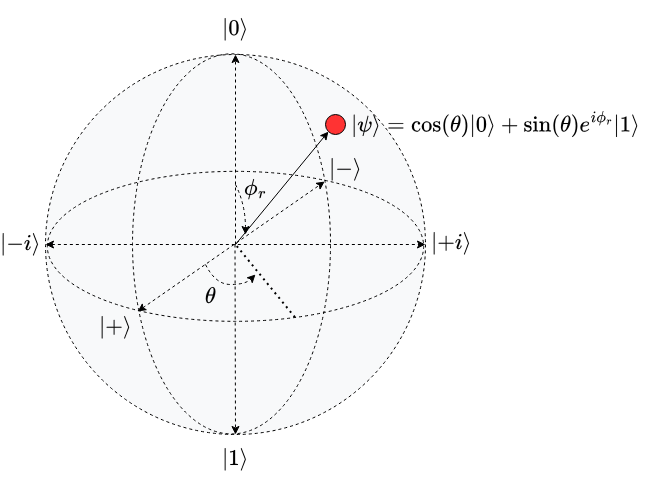
\includegraphics[width=0.80\linewidth]{body/ch2/figs/blochsphere}
	\caption[Bloch sphere diagram representing the quantum state of a qubit as a vector in Hilbert space.]{Showing a Bloch sphere diagram where relative phase is mapped to the vertical rotation around the $xy$-plane and $\theta$ corresponds the angle of the horizontal rotation of the qubit around the $\hat{z}$-axis.}
	\label{fig:blochsphere}
\end{figure}
The Bloch sphere is centred at the origin with a radius of 1. The absolute phase $\theta$ is taken with respect to the $\hat{z}$-axis corresponding to the orthogonal basis vectors, $\ket{0}$ and $\ket{1}$, of the state space. The relative phase $\phi$ is considered with respect to the $\hat{x}$-axis. Generally, each axis of the 3D plane represents two counter states. The states on the $\hat{z}$-axis correspond to the basis vectors,
\begin{align}
	\ket{0}	= \left(\begin{matrix}
		1\\
		0
	\end{matrix}\right) &, 	\ket{1}	= \left(\begin{matrix}
	0\\
	1
\end{matrix}\right)\nonumber
\end{align}
The $\hat{x}$-axis represents the EPR pair, or Bell states, namely,
\begin{align}
		\ket{+}	& = 
		\frac{1}{\sqrt{2}}\left(\begin{matrix}
										1\\
										0
								\end{matrix}\right) + 
		\frac{1}{\sqrt{2}}\left(\begin{matrix}
										0\\
										1
								\end{matrix}\right)\nonumber\\
		\ket{-}	& = 
		\frac{1}{\sqrt{2}}\left(\begin{matrix}
										1\\
										0
								\end{matrix}\right) - 
		\frac{1}{\sqrt{2}}\left(\begin{matrix}
										0\\
										1
								\end{matrix}\right)\nonumber
\end{align}
Similarly, the $\hat{y}$-axis represents the imaginary part of the state vector, or mathematically,
\begin{align}
	\ket{+i}	& = 
	\frac{1}{\sqrt{2}}\left(\begin{matrix}
		1\\
		0
	\end{matrix}\right) + 
	\frac{i}{\sqrt{2}}\left(\begin{matrix}
		0\\
		1
	\end{matrix}\right)\nonumber\\
	\ket{-i}	& = 
	\frac{1}{\sqrt{2}}\left(\begin{matrix}
		1\\
		0
	\end{matrix}\right) - 
	\frac{i}{\sqrt{2}}\left(\begin{matrix}
		0\\
		1
	\end{matrix}\right)\nonumber
\end{align}
Every point on the surface of a Bloch sphere represents a quantum state. This makes Bloch sphere diagrams a very powerful tool for representing quantum gate transformations applied to a qubit.

\subsection{Single-Qubit Quantum Gates\label{subsec:single-q-gates}}

Applications of quantum information processing employs single qubit gates as more of a mathematical abstraction compared to realisable classical logic gates. Quantum gates are not always physically but are extensively used in analysing quantum computing algorithms. From a mathematical point of view, quantum gates are unitary transformations on a small number of qubits. Typically, quantum gates work with up to 3 qubits. 

Single qubit gates correspond to unitary operations known as \textit{Pauli} matrices, I, X, Y, and Z. The Pauli-\texttt{X} gate is analogous to a classical \texttt{NOT} gate in that it performs a qubit flip transformation. For example, given an initial observation of the state $\psi$ which is specified by normalised amplitudes $\alpha$ and $\beta$, the \texttt{X} gate acts linearly to interchange the amplitude of the coefficients that define the superposition by the transformation
\begin{align}
	\texttt{X}: & \ket{\psi}\rightarrow\ket{\psi'}
\end{align}
for 
\begin{align}
	\ket{\psi} & = \alpha\ket{0} + \beta\ket{1}\nonumber\\
	\ket{\psi'} & = \alpha\ket{1} + \beta\ket{0}
\end{align}
The unitary matrix representing the X gate transformation is written as
\begin{align}
	X	& = \left(\begin{matrix}
		0 & 1\\
		1 & 0
	\end{matrix}\right)
\end{align}
Thus, given a qubit in Hilbert space $H_2$ with normalised amplitudes $\alpha$ and $\beta$, the output of the \texttt{X} gate unitary operator is
\begin{align}
	X	\left(\begin{matrix}
	\alpha\\
	\beta
\end{matrix}\right) & = 
\left(\begin{matrix}
	\beta\\
	\alpha
\end{matrix}\right)
\end{align}
This transformation can also be illustrated on a Bloch sphere as shown in figure \ref{fig:xgatebloch} where the initially measured state of the qubit, $\ket{\psi_1}$, is rotated around the $\hat{x}$-axis by $\pi~\si{\radian}$ to obtain $\ket{\psi_2}$. 
\begin{figure}[ht!]
	\centering
	\begin{subfigure}[b]{0.28\textwidth}
		\centering
		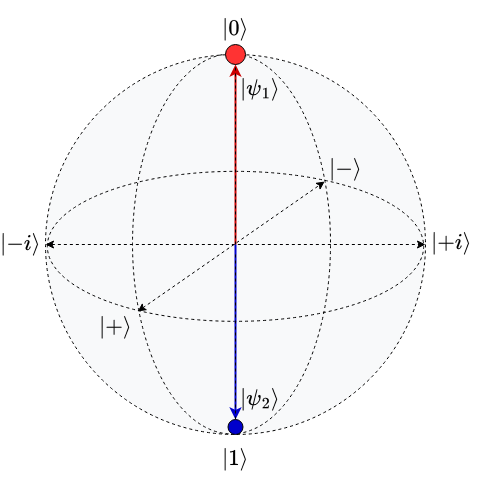
\includegraphics[width=0.9\textwidth]{body/ch2/figs/x-gate}
		\caption{Pauli-\texttt{X} gate.}
		\label{fig:xgatebloch}
	\end{subfigure}
	\hfill
	\begin{subfigure}[b]{0.28\textwidth}
		\centering
		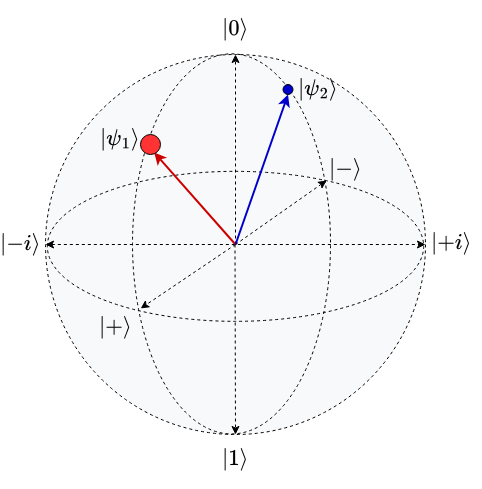
\includegraphics[width=0.9\textwidth]{body/ch2/figs/z-gate}
		\caption{Pauli-\texttt{Z} gate.}
		\label{fig:zgatebloch}
	\end{subfigure}
	\hfill
	\begin{subfigure}[b]{0.28\textwidth}
		\centering
		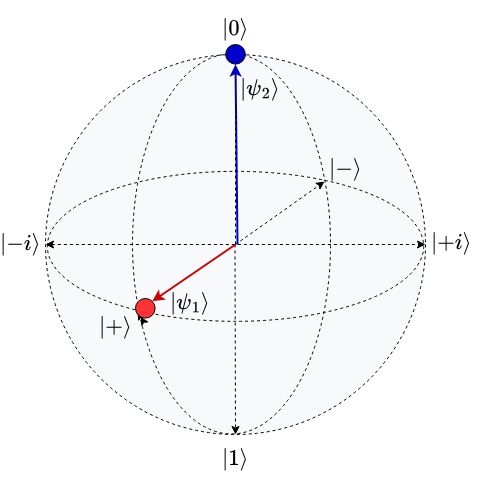
\includegraphics[width=0.9\textwidth]{body/ch2/figs/hadamard-gate}
		\caption{Hadamard (\texttt{H}) gate.}
		\label{fig:hadamardbloch}
	\end{subfigure}
	\caption{Three Bloch spheres representing important single-qubit quantum gate operations. The initial state is in red and the final measured state is blue. The \texttt{X} gate is analogous to a classical \texttt{NOT} gate and the \texttt{Z} gate changes the phase of the qubit.}
	\label{fig:qgates}
\end{figure}

Since the quantum gate is a unitary operator, it maintains the condition of normalisation on the Hilbert space \cite{Nielsen2010}. Other Pauli gate matrices are expressed in equation \ref{eqn:pauligates} where it can be shown that for each unitary matrix $U$, $UU^\dagger=I$, where $U^\dagger$ is the adjoint of $U$. This implies that the identity matrix $I$, operates in a manner that is analogous to a classical circuit buffer which has the same bit at input and output. Applying the an identity gate is equivalent to measuring the same state at the start and end of a computation, the input state of the quantum system is the same as the output state. 
\begin{align}\label{eqn:pauligates}
	I=\left(\begin{matrix}
		1	& 0\\
		0	& 1
	\end{matrix}\right)&;~Y=\left(\begin{matrix}
	0	& -i\\
	i	& 0
\end{matrix}\right)\nonumber\\
Z=\left(\begin{matrix}
1	& 0\\
0	& -1
\end{matrix}\right)&;~H=\frac{1}{\sqrt{2}}\left(\begin{matrix}
1	& 1\\
1	& -1
\end{matrix}\right)
\end{align}
The \texttt{X} gate is one of three physically realisable single-qubit gates that are considered in this research. The other two gates that are of significance to quantum information processing are the Pauli-$Z$ gate and the \textit{Hadamard} gate \texttt{H} - illustrated using Bloch diagrams as shown in figure \ref{fig:zgatebloch} and \ref{fig:hadamardbloch}, respectively. 

Equation \ref{eqn:pauligates} shows that the $Y$ gate performs rotations through the $\hat{y}$-axis which corresponds to the complex plane and is therefore not physically realisable. The \texttt{Z} gate is a special case of the \textit{phase gate},
\begin{align}
	R_\phi	& = \left(\begin{matrix}
		1	& 0\\
		0	& e^{i\phi}
	\end{matrix}\right)
\end{align}
which rotates the state vector of a qubit through the $\hat{z}$-axis by $\phi=\pi~\si{\radian}$, effectively negating the amplitude of the $\ket{1}$ basis state and leaving the $\ket{0}$ basis state unchanged. The Hadamard gate \texttt{H} rotates the qubit by $\pi/2~\si{\radian}$ through the $\hat{y}$-axis and by $\pi~\si{\radian}$ in the $\hat{x}$-axis.  

This implies that, given an initial state $\ket{0}$ to which the Hadamard gate is applied, there is an equal probability of observing $\ket{0}$ or $\ket{1}$ \cite{DeWolf2019}. When a Hadamard gate is applied to the $\ket{+}$ state, the output is derived from
\begin{align}
	H\ket{+} & = H\left[\frac{1}{\sqrt{2}}\left(\begin{matrix}
						1\\0
	\end{matrix}\right) + \frac{1}{\sqrt{2}}\left(\begin{matrix}
	0\\1
\end{matrix}\right)\right]\nonumber\\
& = \frac{1}{\sqrt{2}}H\left(\begin{matrix}
	1\\0
\end{matrix}\right) + \frac{1}{\sqrt{2}}H\left(\begin{matrix}
	0\\1
\end{matrix}\right)\nonumber\\
& = \frac{1}{2}\left(\begin{matrix}
	1\\0
\end{matrix}\right) + \frac{1}{2}\left(\begin{matrix}
	0\\1
\end{matrix}\right) + \frac{1}{2}\left(\begin{matrix}
1\\0
\end{matrix}\right)  \frac{1}{2}\left(\begin{matrix}
0\\1
\end{matrix}\right)\nonumber
\end{align}
which gives the state $\ket{0}$. This derivation of the Hadamard operation exposes the phenomenon of \textit{interference} that qubits experience due to their wave nature. This occurs when the $\ket{1}$ and $-\ket{1}$ states cancel each other out, corresponding to an overlap in the peaks and troughs of the qubit waveforms that are in a superposition of states.

When simulating single-qubit quantum gates, the Hadamard gate is off particular interest since it increases the entropy of the classical computer running the simulation. For this reason, models of the Hadamard gate on the FPGA were expected to use more logic and slices than other single-input quantum gates. Other single-qubit gates can be performed using LUT-multipliers and simple combinational logic operations. 
 
\subsection{Multiple-Qubit Gates\label{subsec:multiple-q-gates}}
Multiple-qubit gates can be realised by performing a sequence of single-qubit gate transformations. Constructing a multiple-qubit gate from two single-qubit systems given by matrix $U$ and matrix $V$ equivalent to taking the tensor product of the matrices, i.e. $U\otimes V$. In some cases, multiple-qubit gates can transform the system such that qubits become entangled. Generally, these type of gates cannot be decomposed into a tensor product of single-bit transformation. An example of a 2-qubit gate is the \textit{controlled}-\texttt{NOT} (\texttt{CNOT}) gate which is defined as the sum of tensor products of the identity matrix \texttt{I} and the \texttt{X} gate with the standard basis inputs $\ket{0}$ and $\ket{1}$, i.e.,
\begin{align}\label{eqn:cnotdef}
	\texttt{CNOT}	&= \ket{0}\bra{0}\otimes I + \ket{1}\bra{1}\otimes X
\end{align}
Equivalently, the unitary matrix representation of the \texttt{CNOT} gate is
\begin{align}\label{eqn:cnotmatrix}
	\texttt{CNOT}	& = \left(\begin{matrix}
		1 & 0  & 0 & 0\\
		0 & 1  & 0 & 0\\
		0 & 0  & 0 & 1 \\
		0 & 0  & 1 & 0
	\end{matrix}\right)
\end{align}
Given a standard basis input, the \texttt{CNOT} gate has four possible outputs, namely,
\begin{align}
	\texttt{CNOT}~~: & \begin{cases}
		\ket{00} \rightarrow \ket{00}\\
		\ket{01} \rightarrow \ket{01}\\
		\ket{10} \rightarrow \ket{11}\\
		\ket{11} \rightarrow \ket{10}	
	\end{cases}
\end{align}
The $\texttt{CNOT}$ gate is particularly important for applications in quantum information processing due to its capability to change the entanglement between input qubits \cite{Rieffel2011}. For example, given the separable 2-qubit input state $\ket{\psi_1}$ where  
\begin{align}
	\ket{\psi_1}	& = \frac{1}{\sqrt{2}}\left(\ket{0} + \ket{1}\right)\otimes\ket{0}
\end{align}
the \texttt{CNOT} gate converts unentangled input state to an entangled Bell state
\begin{align}
	\ket{\psi_2} 	& = \frac{1}{\sqrt{2}}\left(\ket{00} + \ket{11}\right)\nonumber
\end{align}
The generalised \texttt{CNOT} gate consists of gates that perform a single-qubit transformation $Q$ on the second qubit in the input when the first input is the basis state $\ket{1}$ and leave it unchanged when the first input is $\ket{0}$. The first input is called the \textit{control qubit} and the second qubit is called the \textit{target qubit}. Formally, the generalised \text{CNOT} gate can be expressed as
\begin{align}
	\Lambda Q	& = \ket{0}\bra{0}\otimes I + \ket{1}\bra{1}\otimes Q
\end{align}
where $Q$ is a $2\times2$ matrix. Thus, the $4\times4$ matrix representation of the generalised \texttt{CNOT} gate is
\begin{align}\label{eqn:generic-cnot}
	\Lambda Q	& = \left(\begin{matrix}
						1	&0	&0	&0\\
						0	&1	&0	&0\\
						0	&0	&q_{11}	&q_{12}\\
						0	&0	&q_{21}	&q_{22}
					\end{matrix}\right)
\end{align}
where each $q_{ij}$, for $i = 1,2$ and $j=1,2$, is an element of the single-qubit gate $Q$. The graphical representation of the generalised \texttt{CNOT} gate and the special case of the \texttt{CNOT} which uses the $X$ gate is shown in figure \ref{fig:cnotDiagram}.
\begin{figure}
	\centering
	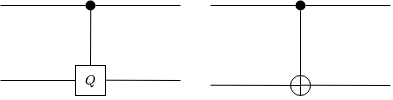
\includegraphics[width=0.75\linewidth]{body/ch2/figs/cnot-diagram}
	\caption[Generalised \texttt{CNOT} gate and the $\Lambda X$ \texttt{CNOT} gate.]{The $\Lambda X$ gate is a 2-qubit gate which is a special case of the generalised 2-qubit $\Lambda Q$ \texttt{CNOT} gate.}
	\label{fig:cnotDiagram}
\end{figure}
Note that the control qubit of the \texttt{CNOT} gate does not change and the target qubit changes depending on the state of the control qubit. This operation is analogous to the operation of the \texttt{XOR} gate, since the unitary transformation can also be expressed algebraically as
\begin{align}
	\texttt{CNOT}: & \ket{A,B} \rightarrow \ket{A, B\oplus A }
\end{align}
where $\oplus$ represents the direct sum of the basis sets $A$ and $B$ that produces a vector space with basis $A\cup B$.

Emulations of controlled gate operations require more area on FPGA hardware than single-qubit gates since they operate on two qubits simultaneously to and require dense matrix operations for large $n$. Additionally, the output of a controlled gate is an entangled state which increases the amount of storage required to represent quantum states on the FPGA hardware. Therefore, the number of controlled gates in a quantum circuit was expected to directly influence the overall performance of the simulation. 

\subsection{Quantum Circuits \label{subsec:q-circuits}}
Illustrations of the \texttt{CNOT} gate as shown in figure \ref{fig:cnotDiagram} form an essential part of representing and interpreting quantum computations. A sequence of quantum gates forms a \textit{quantum gate array}, also known as a \textit{quantum circuit}. Quantum circuits are a universal language for describing complex quantum computations \cite.  In a quantum circuit, single-qubit gates are represented using block diagram notation as depicted in figure \ref{fig:gatecircuitcomponents}. In 1995, Barenco et al. proved that arbitrary quantum circuits can be expressed by compositions of a set of single-qubit gates and \texttt{CNOT} gates \cite{barenco1995elementary}. Furthermore, since there are infinitely many $2\times2$ unitary matrices, there are also infinitely many single-qubit gates and quantum circuits. 
\begin{figure}[!ht]
	\centering
	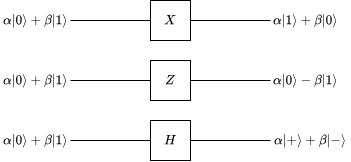
\includegraphics[width=0.85\linewidth]{body/ch2/figs/single-qubit-components}
	\caption[Showing the circuit representation of quantum $X$, $Z$ and $H$ gates.]{Quantum circuit gate component representations of the Pauli-$X$, Pauli-$Z$ and $H$ single-qubit logic gates.}
	\label{fig:gatecircuitcomponents}
\end{figure}
In quantum circuit representations, time progresses from the input of the quantum circuit on the left, to the right which terminates in a measurement of the output state. Each line in the quantum circuit represents a wire, which in turn, represents the passage of time from left to right or a qubit of information as it is translated in Hilbert space. By convention, it is assumed that the multiple-qubit input to a circuit is the state consisting of a sequence of $\ket{0}$ basis states. It is crucial to note that the final state of an input qubit cannot be determined by only looking at the wire corresponding to that qubit. For example, from the circuit in figure \ref{fig:hadamard2circuit}, 
\begin{figure}[!ht]
	\centering
	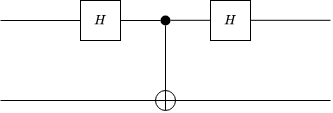
\includegraphics[width=0.75\linewidth]{body/ch2/figs/q-circuit-caution}
	\caption[The output of a qubit cannot be accurately determined by looking at a single line in a quantum circuit.]{Demonstrating a quantum circuit that consists of two series $H$ gates on the control line of the $\Lambda X$ gate.}
	\label{fig:hadamard2circuit}
\end{figure}
it might appear that the first qubit's state would remain the same since $H^2 = I$, however, given the input state $\ket{00}$, the state of the output is defined by the unitary transformation
\begin{align}
	U: & \ket{00} \rightarrow \frac{1}{2}\left(\ket{00} + \ket{10} + \ket{01} - \ket{11}\right) \nonumber
\end{align}
which is not obvious by focusing on the control line of the circuit \cite{Rieffel2011}. Figure \ref{fig:swapcircuit} shows another example of a quantum circuit known as a \textit{swap gate} which contains three \texttt{CNOT} gates. Since the \texttt{swap} gate uses \texttt{CNOT} gates, it follows a sequence of transformations on a basis state $\ket{\psi_a, \psi_b}$ that involves direct sums of vector states that produces an output where the qubit states are interchanged. The \texttt{swap} gate uses both qubits as the control to perform the operation
\begin{align}
	\ket{\psi_a, \psi_b}	&\rightarrow \ket{\psi_a, \psi_a\oplus \psi_b}\nonumber\\
				&\rightarrow \ket{\psi_a\oplus (\psi_a\oplus \psi_b), \psi_a\oplus \psi_b}\nonumber\\
				& = \ket{\psi_b, \psi_a\oplus\psi_b}\nonumber\\
				& \rightarrow \ket{\psi_b, (\psi_a\oplus\psi_b)\oplus\psi_b}\nonumber\\
				& = \ket{\psi_b, \psi_a}
\end{align}
The \texttt{swap} gate is also equivalent to applying the transformation $U$, given by,
\begin{align}
	U: & \ket{\psi_a}\bra{\psi_a}\otimes X	+ \ket{\psi_b}\bra{\psi_b} \otimes X
\end{align}
which applies a tensor product of the Pauli-$X$ gate to each qubit in the system. 
\begin{figure}[!ht]
	\centering
	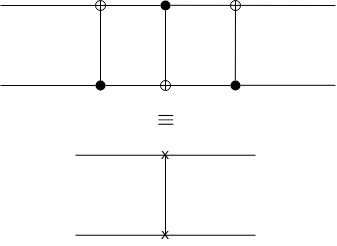
\includegraphics[scale=0.55]{body/ch2/figs/swap-circuit}
	\caption[Swap gate interchanges input qubits in a 2-qubit system.]{Quantum circuit of a \texttt{swap} gate that interchanges the input state from $\ket{\psi_a,\psi_b}$ to $\ket{\psi_b,\psi_a}$.}
	\label{fig:swapcircuit}
\end{figure}
Quantum circuits are said to be \textit{acyclic} in that feedback from one part of the circuit to another is prohibited \cite{Rieffel2011}. This is contrary to classical electronic circuits which employ feedback to control the stability of classical systems. Another contradiction between quantum circuits and classical circuits is that quantum circuit wires cannot be joined together to perform an operation that is analogous to a classical \texttt{OR} gate operation. Additionally, most quantum circuit operations are reversible since they use unitary operations, however, duplication of qubit states is prohibited according to the \textit{no-cloning theorem}, which implies that copy operations at the output of a quantum circuit are prohibited.  

Quantum circuit outputs are measured to collapse the single qubit state $\ket{\psi}$ with basis states $\ket{0}$ and $\ket{1}$ to a classical bit $\sigma$ where the probability of obtaining $0$ is $|\alpha|^2$ and the probability of obtaining 1 is $|\beta|^2$, such that the normalisation condition is satisfied. The symbol for a measurement in a quantum circuit is shown in figure \ref{fig:measurement-symbol} where $\sigma$ is represented by a double-line wire. 
\begin{figure}[!ht]
	\centering
	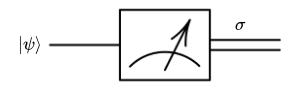
\includegraphics[width=0.70\linewidth]{body/ch2/figs/measurement-symbol}
	\caption[Quantum circuit measurement symbol.]{Quantum circuit measurement symbol.}
	\label{fig:measurement-symbol}
\end{figure}
A measurement on a multidimensional qubit (sometimes referred to as a "qudit") collapses the superposition of states to a single classical $n$-bit configuration that is chosen randomly with probability that satisfies the normalisation condition on the amplitudes of each state. A measurement can also be viewed as an interface that converts quantum information to classical information. By the no-cloning theorem, measurements of the output of a quantum circuit are irreversible as the quantum information is destroyed when the superposition of states collapses into a single classical bit or strings of classical bits. One way around the no-cloning theorem is to implement teleportation and quantum error-correction in which information about the quantum state being measure is concealed. 
 
\textit{Circuit depth} refers to the count of time steps from the initialisation of the qubits to the final measurement taken. In determining the circuit depth, all gates executed in parallel count as one time step, including cases where the execution times of each gate are significantly different \cite{de2021reducing}. Analogously, the critical path of FPGA designs refers to the longest sequence of logic gates that data must pass through and the latency of the digital circuit. In designing the simulation of quantum gates on FPGA, the aim is to reduce the critical path by parallelising operations involving multiple qubit gates such as the controlled gate. For FPGAs however, the critical path includes pipeline registers for storing quantum state evolutions during the execution of a quantum circuits simulations.

\subsection{Theoretical Framework for Quantum Algorithms \label{subsec:qft}}

In quantum computing, \textit{quantum algorithms} are executed using quantum circuits. During the proposal of elementary gates for quantum computing, Barenco et al. suggested that most quantum algorithms can be decomposed into a combination of single-qubit gates such as the previously described Pauli gates and two-qubit \texttt{CNOT} gates represented as $2^n \times 2^n$ dense matrices \cite{barenco1995elementary}. Applying unitary quantum gates to qubits in a quantum circuit transforms the $2^n$ complex entries of the $n$-qubit state vector, corresponding to a multiplication of the qubit state vector with the unitary matrix of the quantum gate \cite{li2019tackling}. To emulate a quantum computer on available classical computers, H\"{a}ner et al. suggest that instead of simulating the vast number of quantum gates required for a quantum computation, one can perform the classical function directly for each computational basis state \cite{haner2016high}. Developed here is the formalism of the Quantum Fourier Transform (QFT) which is the primary quantum circuit in Shor's quantum factoring algorithm and other quantum algorithms. The mathematical formalism of the \textit{quantum search algorithm}, also known as \textit{Grover's search algorithm}, is also considered in this section. Understanding of these algorithms is critical in the emulation of the quantum computer on FPGA. 

\subsubsection{Quantum Fourier Transform \label{subsubsec:qft}}

In the analysis of linear time-dependent classical systems, the Fourier transform is harnessed as a reversible tool that transforms a signal from the time domain to the frequency domain and vice versa. In the discrete time domain, the Fast Fourier transform (FFT) is performed to reduce the computational complexity by decomposing the Discrete Fourier transform (DFT) of a signal into two half-point transforms. In quantum computing, the QFT is the quantum counterpart of classical DFT algorithms. A 3-qubit QFT circuit demonstrated by Nielsen and Chuang, uses a sequence of \texttt{H} gates, $\texttt{R}_\phi$ phase gates, and a special case of the phase gate known as the \texttt{T} gate which rotates a state vector by $\phi=\pi/8~\si{\radian}$. For an $n$-qubit system, a total of $n(n+1)/2+n/2$ gates are required to perform the QFT \cite{Nielsen2010}. Since each quantum gate transformation involves matrix multiplication and vector addition operations, simulations of the QFT require intensive computational resources. This high performance capabilities of FPGAs makes them suitable for performing quantum experiments using a simulation of the QFT. 
\begin{figure}[!ht]
	\centering
	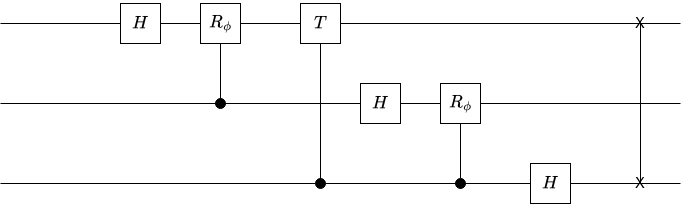
\includegraphics[width=1.0\linewidth]{body/ch3/figs/nielsen-qft}
	\caption[Nielsen 3-qubit QFT.]{An explicit quantum circuit for the 3-qubit Quantum Fourier Transform which uses the Hadamard gate, $H$, phase gate, $R_\phi$, and the $\pi/8$ gate, $T$.}
	\label{fig:nielsen-qft}
\end{figure}
Formally, the QFT on the basis $\ket{0}, \ket{1}, ...,\ket{N-1}$ is defined to be a linear operator with the following transformation on the vector space, 
\begin{align}\label{eqn:qft}
	\ket{j}	& \rightarrowtail \frac{1}{\sqrt{N}} \sum_{k=0}^{N-1} e^{2\pi i j k/N}\ket{k}
\end{align}
which is a unitary transformation that can be implemented using a quantum computer \cite{Nielsen2010}. Note the state $\ket{j}$ can be written in the binary representation $j = j_1j_2...j_n$. It can be shown that the QFT is a unitary transformation by expanding the definition. Let $N=2^n$, where $n$ is an integer, and let the basis $\ket{0},...,\ket{2^n - 1}$ be the computational basis for an $n$ qubit quantum computer \cite{Nielsen2010}. By expressing the binary fraction 
\begin{align}
	\frac{j_l}{2} + \frac{j_{l+1}}{2} + ... +\frac{j_{m}}{2^{m-l+1}} \nonumber
\end{align}
in the notation $0.j_lj{l+1}...j_{m}$, where $l = 1,2,..,n$, the QFT can expanded as the product representation as
\begin{align}\label{eqn:qft-product}
	\ket{j_1\cdots j_n} & \rightarrowtail	\frac{(\ket{0} + e^{2\pi i 0.j_n}\ket{1})(\ket{0} + e^{2\pi i 0.j_{n-1}j_n}\ket{1})}{2^{n/2}} \nonumber\\
	& \frac{\cdots(\ket{0}+ e^{2\pi i 0.j_1j_2\cdots j_n}\ket{1})}{2^{n/2}}
\end{align}
which is a linear action on the state $\ket{j}$ which exploits the properties of distributivity and commutativity of the Hadamard and $R_\phi$ gate unitary transformation as illustrated in the 3-qubit QFT quantum circuit in figure \ref{fig:nielsen-qft} above. The product representation of the QFT is useful in emulations of quantum computers because, unlike simulations with increased overhead from modelling all the gates, emulators can perform execute quantum algorithms in the computational basis \cite{haner2016high}. 

As an example, consider the case where $n=3$. The QFT 3-qubit product representation of the QFT is,
\begin{align}\label{eqn:qft-3-qubit-example}
	\ket{j_1j_2j_3}	& = \frac{1}{\sqrt{2}}\left(\ket{0} + e^{2\pi i 0.j_3}\ket{1}\right)\nonumber\\
	& \otimes\frac{1}{\sqrt{2}}\left(\ket{0} + e^{2\pi i 0.j_2j_3}\ket{1}\right)\nonumber\\
	& \otimes\frac{1}{\sqrt{2}}\left(\ket{0} + e^{2\pi i 0.j_1j_2j_3}\ket{1}\right)
\end{align}
 
The corresponding matrix for the \texttt{QFT} gate described by the 3-qubit quantum circuit in figure \ref{fig:nielsen-qft} is written explicitly, using $\omega = e^{2\pi/8}$, as
\begin{align}\label{eqn:qft-matrix}
	\texttt{QFT}	& = \frac{1}{\sqrt{8}}\left(\begin{matrix}
		1 & 1 & 1 & 1 & 1 & 1 & 1 & 1\\
		1 & \omega & \omega^2	& \omega^3	& \omega^4	& \omega^5	& \omega^6	&	\omega^7\\
		1 & \omega^2 & \omega^4	& \omega^6	& 1	& \omega^2	& \omega^4	&	\omega^6\\
		1 & \omega^3 & \omega^6	& \omega^1	& \omega^4	& \omega^7	& \omega^2	&	\omega^5\\
		1 & \omega^4 & 1	& \omega^4	& 1	& \omega^4	& 1	&	\omega^4\\
		1 & \omega^5 & \omega^2	& \omega^7	& \omega^4	& \omega	& \omega^6	&	\omega^3\\
		1 & \omega^6 & \omega^4	& \omega^2	& 1	& \omega^6	& \omega^4	&	\omega^2\\
		1 & \omega^7 & \omega^6	& \omega^5	& \omega^4	& \omega^3	& \omega^2	&	\omega^1
	\end{matrix}\right)
\end{align}

In the first stage of the QFT circuit shown in figure \ref{fig:nielsen-qft}, a Hadamard gate is applied to the first register $\ket{j_3}$, giving the transformation,
\begin{align}\label{eqn:qft-step-1}
	\ket{j_3} &	\rightarrowtail \frac{1}{\sqrt{2}}\left(\ket{0} (-1)^{0.j_3}\ket{1}\right)
\end{align}
In the next time step, a controlled-$R_\phi$ gate operation is applied to the $\ket{j_2}$ such that the \gls{ancilla} matrix of the controlled-gate is raised to successive powers of two \cite{Nielsen2010}. This is accomplished by applying the controlled $R_\phi$ gate before a Hadamard gate operation is executed on $\ket{j_2}$, yielding,
\begin{align}\label{eqn:qft-step-2}
	\ket{j_2}	& \rightarrowtail \frac{1}{\sqrt{2}}\left(\ket{0} (-1)^{0.j_2j_3}\ket{1}\right)
\end{align}
The second stage of the QFT is equivalent to applying the inverse QFT to the first register $\ket{j_3}$.  The output on the third wire gives the state
\begin{align}\label{eqn:qft-step-3}
	\ket{j_1}	& \rightarrowtail \frac{1}{\sqrt{2}}\left(\ket{0} (-1)^{0.j_1j_2j_3}\ket{1}\right)
\end{align}
The first qubit should be in the third position and vice versa, which can be achieved by applying a \texttt{swap} gate at the output of the first and last registers \cite{DeWolf2019}. In this paper, the general case for a quantum computer with $n$-qubits was expected to use $\mathcal{O}(n\log n)$ gates overall for computing the QFT. This is because the contribution of the controlled-$R_\phi$ gate is equivalent to the $I$ gate which has a negligible contribution to the total number of gate \cite{DeWolf2019}.

\subsubsection{Phase Estimation and Shor's Factoring Algorithm \label{subsubsec:q-shors-algo}}

The objective of QFT implementations is not to speed up Fourier transforms of time-dependent wave functions. Rather, the QFT allows for \textit{phase estimation}, i.e., approximation of the eigenvalues of a unitary operator \cite{Nielsen2010}. Phase estimation is approached as a modular part of an algorithm such that when combined with other subroutines, the module can perform quantum parallel tasks \cite{Nielsen2010}. Phase estimation uses black boxes, or \textit{quantum oracles} which are capable of preparing an unknown quantum state and performing a controlled-gate operation. A quantum oracle is a unitary $U$ with an eigenvector $\ket{\sigma}$ and corresponding eigenvalue $\lambda$, i.e.
\begin{align}
	U\ket{\sigma} & = \lambda\ket{\sigma}\nonumber 
\end{align}
Since the oracle is a unitary operation, $\lambda = 1$, which can be written as the exponential function $e^{2\pi i \Phi}$, for some phase $\Phi~\in~[0,1)$. To produce the correct phase estimate, the state of the oracle is read out in the third and final stage of the QFT circuit to give a good estimate of the phase \cite{Nielsen2010}. In the ideal case where the phase $\Phi$ can be written with exactly $n$ bits of precision, the inverse QFT produces the exact phase from $\ket{2^n\Phi} = \ket{\Phi_1\Phi_2\cdots\Phi_n}$ with probability 1 \cite{DeWolf2019}. In cases where this condition does not hold, the QFT produces a good estimate of the phase. Classical implementations of quantum oracles use two registers, one containing $m$ qubits that are initially in the state $\ket{0}$ and a second register which begins in the state $\ket{\psi_u}$, and contains as many qubits as is necessary to represent the state. Assuming that the first register is prepared in $t$ qubits such that
\begin{align}\label{eqn:phase-estimation-t}
	t & = 2L + 1 + \lceil\log\left(2 + \frac{1}{2\epsilon}\right)\rceil
\end{align}
where $0<\epsilon|< 1$ and $L \equiv \lceil \log N\rceil$, and the second register is prepared in the state $\ket{1}$, then it follows that for each $s$ such that $0 < s < r - 1$, the estimate of the phase is $\Phi \approx s/r$, accurate to $2L+1$ bits, with probability (1-$\epsilon$) \cite{Nielsen2010}. Phase estimation using the QFT forms part of the solution to many problems including order-finding and factoring problems.

In a 1994 seminal paper, Shor introduced quantum order-finding algorithms as an effective means for solving discrete logarithms and factoring problems \cite{Shor1994}. Most applications of Shor's algorithm involve the use the QFT circuit in combination with other gates such as the Hadamard gate \cite{Zhang2019, Hlukhov2021}. Shor's factoring algorithm can find a factor of a composite number $N$ in roughly $\mathcal{O}(\log\log N)$ steps using a similar concept to the application of phase estimation using the QFT for computing the \textit{order} of a positive integer $x$ that is \gls{co-prime} to the positive integer $N$, such that $x < N$. The \textit{order} of $x$ modulo $N$ is defined to be the least positive integer $r$, such that $x^r = 1(\text{mod}N)$. The order of an element $x$ can be found by noting that the sequence 
\begin{align}
	1,x^1(\text{mod}N),~~x^2(\text{mod}N),~...\nonumber
\end{align}
cycles with period $r$ such that $0 < r \leq N$. Formally, the order-finding problem aims to find the value of $r\in {0,...,N-1}$ such that for the function $f:\mathbb{N} \rightarrow {0,...,N-1}$,  $f(a) = f(b)$ if and only if $a=b~\text{mod}~r$ \cite{DeWolf2019}.  

Classical computers cannot solve the ordering-problem efficiently for large values of $r$. It can be shown that this problem can be solved efficiently on a quantum computer with only $\mathcal{O}(\log\log N)$ evaluations of function $f$ and $\mathcal{O}(\log\log N)$ QFT transforms \cite{DeWolf2019}. The aim of this project is to perform quantum algorithms using the emulated quantum computer which offers polynomial runtime. Shor's factoring algorithm finds the prime factors of an $L$-bit integer $N$ in $\mathcal{O}(L^3)$ operations reducing the order-finding subroutine to computing the period of a random number $x$ \gls{co-prime} with $N$ \cite{Nielsen2010}. The input to the factoring algorithm is a composite number $N$ and the output is a non-trivial factor of $N$. In the first step, the algorithm assesses the parity of the input $N$, i.e. if $N$ is even, then the factor 2 is returned. In the following step, if $N = a^b$ for integers $a\geq1$ and $b\geq2$, then the factor $a$ is returned using the product expansion of the QFT in the computational basis. The value of $x$ is randomly chosen in the range between 1 and $N-1$ such that if the greatest common divisor between $x$ and $N$ is greater than 1, then the greatest common divisor is returned as a factor of $N$ \cite{Nielsen2010}. The order-finding subroutine is used to find the order $r$ of $x$ modulo $N$ such that if $r$ is even and $x^{r/2} \neq -1(\text{mod}N)$, then the greatest common divisors between $x^{r/2} - 1$ and $N$, as well as $x^{r/2} + 1$ and $N$ are computed in order to compare the outputs and identify the correct factor. The quantum factoring algorithm succeeds in finding the factors of $N$ with probability $\mathcal{O}(1)$ \cite{Nielsen2010}.  

There is no known classical algorithm that can factor a composite number $N$ polynomial time. In this paper, an FPGA is used to emulate a quantum computer which performs Shor's algorithm for factoring composite numbers in polynomial time. The quantum computing emulator is designed to perform Shor's algorithm, as welll as the QFT and order-finding routines in the computational basis. The following section establishes the theoretical framework for performing quantum search algorithms using the QFT quantum circuit subroutine.

\subsubsection{Quantum Search Algorithm \label{subsubsec:q-search-algo}}

The quantum search algorithm, which is also known as Grover's search algorithm, offers a quadratic speedup in searching a database or search space with $N$ entries. Given $N = 2n$ and an arbitrary value $x \in \{0, 1\}^N$, the search problem is to find an $i$ such that $x_i = 1$ \cite{DeWolf2019}. The search problem can also be represented by a function $f$ with positive integer input $x < N$. If $x$ is a solution to the search problem, then the output of $f$ is 1, otherwise the output is 0. The number of solutions in $x$ is denoted by $\mu$. The quantum search algorithm is used to find the shortest-path between the nodes of a graph and speedup \gls{NP-complete} problems. The advantage of using the quantum search algorithm is that it solves the search problem in $\mathcal{O}(\sqrt(N))$ entries and using $\mathcal{O}(\sqrt{N}\log N)$ gates whereas a classical search algorithm would require $\mathcal{O}(N)$ queries to solve the search problem. When traversing the search space of $N$ items, the algorithm uses the indices of the elements modelled by an $N$-bit string. At the start, the registers are initialised to the state $\ket{0^n}$ and a Hadamard gate is applied to each qubit to obtain the uniform superposition
\begin{align}
	\ket{U} & = \frac{1}{\sqrt{N}}\sum_{j}\ket{j}
\end{align}
of all the indices in the search space. A quantum oracle $\Omega$, is used to recognise solutions to the problem using an action on the computational basis denoted by
\begin{align}\label{eqn:grovers-oracle}
	\Omega: & \ket{x}\ket{q} \rightarrow \ket{x}\ket{q\oplus f(x)}
\end{align}
where $x$ is the index register, $\oplus$ is addition modulo 2, and $\ket{q}$ is a single qubit which is flipped if $f(x) = 1$, and remains 0 otherwise. The quantum search algorithm prepares the state $\ket{x}\ket{0}$ and applies the oracle with the oracle qubit initially in the state 
\begin{align}
	\ket{q}	& = \frac{1}{\sqrt{2}}\left(\ket{0} - \ket{1}\right)\nonumber
\end{align}
which gives equal probability of obtaining $\ket{0}$ or $\ket{1}$. If $x$ is a solution, then $\ket{0}$ and $\ket{1}$ are interchanged. The state of the qubit does not change throughout the procedure of the quantum search algorithm, which implies that the action of the oracle can be expressed as
\begin{align}
	\ket{x} \rightarrow (-1)^{f(x)}\ket{x}
\end{align} 
which represents a shift in the phase of the solution. For $\mu$ solutions of $x$, the oracle is applied $\mathcal{O}(\sqrt{N/M})$ times during the execution of the algorithm on a quantum computer. The repeated application of the subroutine $G$ consisting of the Hadamard and oracle $\Omega$ gates is known as \textit{Grover's iterate}. The quantum circuit which uses Grover's iterate to complete the quantum search algorithm is shown in figure \ref{fig:grover-quantum-circuit}. 

\begin{figure}[!ht]
	\centering
	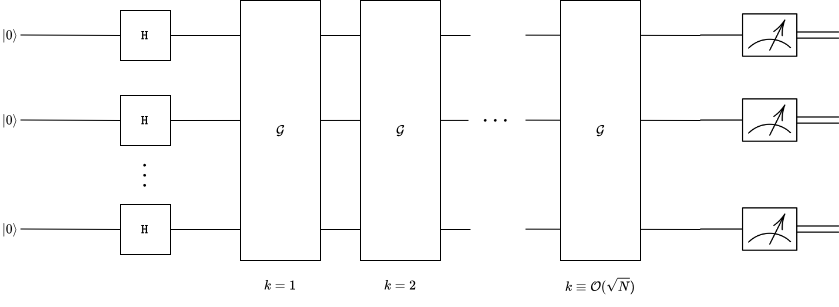
\includegraphics[width=1.0\linewidth]{body/ch2/figs/grovers-quantum-circuit}
	\caption[Generalised Quantum Circuit for Applying Grover's Search Algorithm with $k$ Iteratives.]{The quantum search algorithm applies $\mathcal{O}(\sqrt{N})$ Grover's iteratives to find the solution $x$ to an arbitrary function $f(x) \in \{0, 1\}^n$.}
	\label{fig:grover-quantum-circuit}
\end{figure}

Applications of the Hadamard and oracle $\omega$ gates can be represented on a Bloch sphere as a rotation of the two-dimensional space spanned by the starting vector and the state consisting of a superposition of the $\mu$ solutions of the solution space. The conditional phase shift on the qubits is applied to every computational basis except for the state $\ket{0}$ which receives a phase shift of -1. Overall, the oracle $G$ can be written as
\begin{align}\label{eqn:grovers-iterate}
	G & = (2\ket{x}\bra{x} - I)\Omega
\end{align}
where $I$ denotes the identity operation \cite{Nielsen2010}. After applying the last iteration $G$, the quantum search algorithm terminates with a measurement of the first $n$ qubits in the output register to obtain the solution $x$.

This paper focuses on an implementation of the quantum search algorithm using an FPGA-based quantum emulator in the computational basis. The implementation focuses on applying the procedure on a search space of size $N = 4$, corresponding to a single round of the Grover's iterative subroutine on a 3-qubit system that finds a two-bit solution $x$. Additionally, the quantum search algorithm is implemented with phase estimation in order to count the number of solutions $\mu$ to the search problem. Additionally, the design of the quantum search algorithm is restricted to structured databases which makes the implementation suitable for applications on sorted search spaces. 
 
\section{Summary \label{sec:ch2-conclusion}}
Quantum gates are unitary operations on vector states that transform the properties of qubits. This mathematical definition of quantum gates is useful in interpreting vector transformations, however, the structures represented in by the mathematics may not always be realisable. For that reason, this paper focuses on quantum gates that are realisable such as the \texttt{X}, \texttt{Z}, \texttt{H}, and \texttt{CNOT} gates. For solid state or optical quantum computers, these unitary transformations on qubits can be physical operations such as the application of a magnetic field to particles in NMR and laser pulses in ion trap implementations\cite{Rieffel2011}. Performing quantum computation can be difficult due to the probabilistic behaviour of qubits, thus, modelling systems that are costly to achieve with current technology can be useful. The theoretical framework formulated in this section forms the foundation to the concepts used to design and emulate a quantum information processing system on FPGA.